\chapter{Heart rate sensor}\label{ch:heartRate}
%**********************************************

%**********************************************
\section{Introduction} \label{sec:heartIntro}
%**********************************************
Circuits pertaining to signal conditioning, pulse signal and analogue output generation will be discussed. Conditioning is done via filtering and amplification; active filters provide high input and low output impedance, and a large Q-factor \cite{actpas}. A differential amplifier is suitable for amplification, as the gain is referenced against a customizable voltage \cite{opamp}. A Schmitt Trigger is well-suited for pulse generation, as it provides a noise margin \cite{schmitt}. PWM signals can be converted to analogue using filtering \cite{PWM}.

%**********************************************
\section{Design} \label{sec:heartDesign}
%**********************************************
\begin{figure}[h]
    \centering
    \vspace{-0.7cm}
    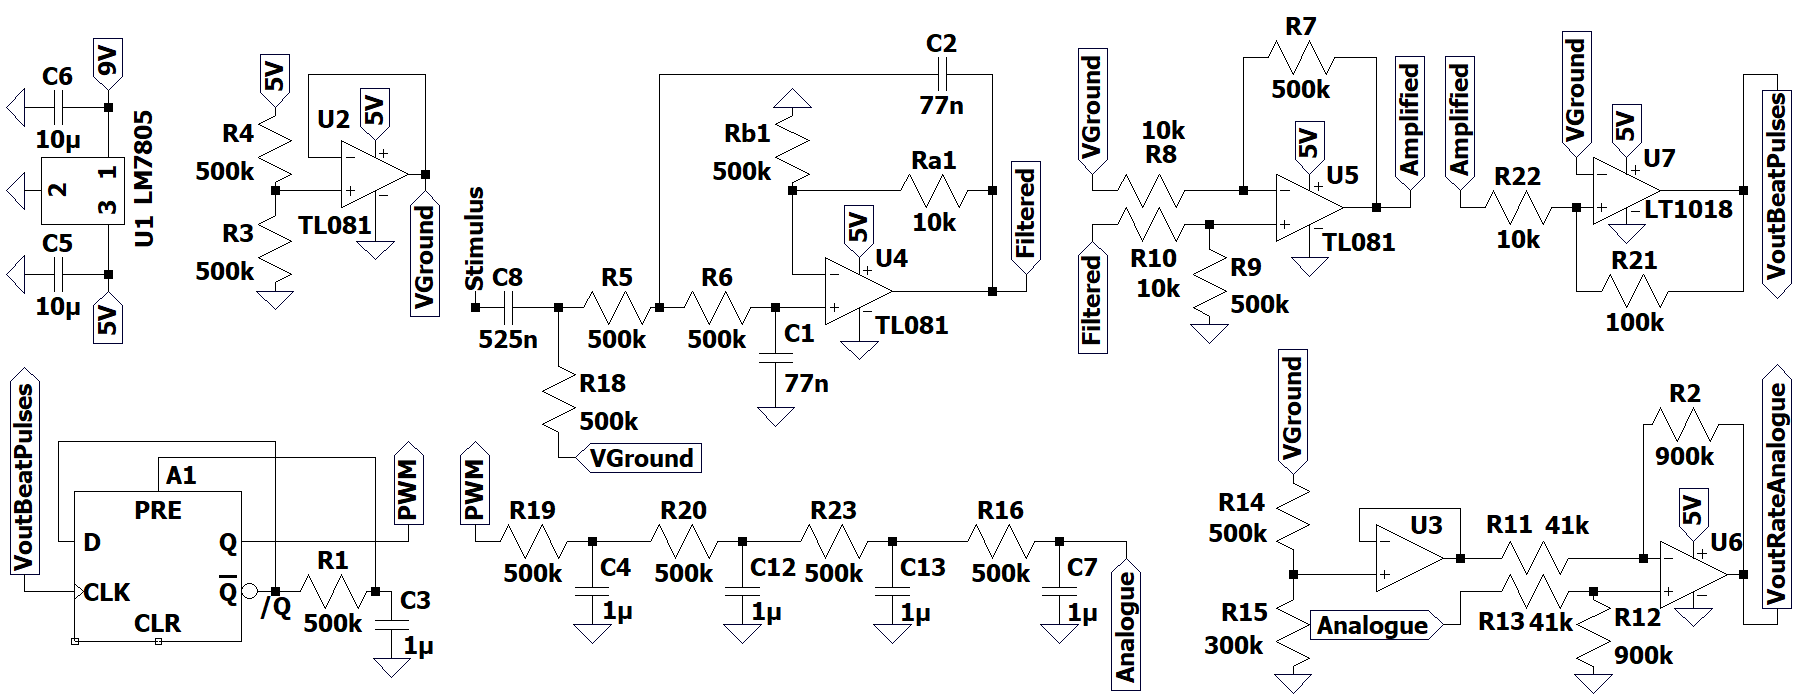
\includegraphics[width = 1\textwidth]{Figures/circuit}
    \caption{Complete Circuit \textbf{enlarge this}}
    \label{fig:circuit}
\end{figure}

The complete circuit is shown upfront in figure \ref{fig:circuit} in order to aid with explanation. Note that when resistor values are selected at random, the largest resistor in the sub-circuit is always chosen to be \SI{500}{k\Omega}, as to reduce current usage. The design process now follows.\\
The stimulus input signal contains noise at \SI{0.25}{Hz} and at \SI{5}{Hz} and higher. The information in the signal resides between \numrange{0.8}{2.5} \si{Hz}, corresponding to 50 and 150 BPM respectively. Noise results in distorted square wave output, thus necessitating filtering. A first order passive high-pass filter, cutoff frequency \SI{0.606}{Hz}, attenuates the low frequency noise. With R18 = \SI{500}{k\Omega}, C8 = \SI{525}{nF} according to $f_{c} = \frac{1}{2\pi R C}$. The capacitor is connected to a virtual ground of \SI{2.5}{V}, thus centering the signal around \SI{2.5}{V}. A second order active low-pass filter, cutoff frequency \SI{4.1}{Hz}, filters out high frequency noise. R5 = R6 = \SI{500}{k\Omega}, C1 = C2 = \SI{77}{nF} - see aforementioned formula. Cutoff frequencies were selected to remove noise maximally while minimally affecting heart-rate data. The signal should reside slightly above \SI{2.5}{V} to facilitate amplification (to be discussed). Thus, Rb1 = \SI{500}{k\Omega} and Ra1 = \SI{10}{k\Omega} since $A_v=1+\frac{R_{A}}{R_{B}}$ 
\cite{filter}. The TL081 op-amp is used, as it is less expensive than the TLC2272 \cite{octo}. A filter output with DC offset slightly above \SI{2.5}{V} allows for the use of a differential amplifier with the existing virtual ground connected to the negative input, thus removing the need for additional circuitry otherwise required to provide a voltage level at the negative input. The signal is amplified according to $\mathrm{V}_{\mathrm{OUT}}=\frac{\mathrm{R}_{a}}{\mathrm{R}_{b}}\left(\mathrm{V}_{2}-\mathrm{V}_{1}\right)$ \cite{opamp}, where R\textsubscript{a} corresponds to R7 and R9, and R\textsubscript{b} to R8 and R10. The gain of 50 was selected to again provide a DC offset of \SI{2.5}{V}, as it facilitates implementation of the comparator (to be discussed). Since the amplified signal has an amplitude of only \SI{1.66}{V}, the inexpensive TL081 was chosen despite having a smaller output range. Next, the signal is fed into a Schmitt Trigger comparator, which produces \SI{5}{V} if the input exceeds the upper trip point (UTP) and \SI{0}{V} if the input falls below the lower trip point (LTP) \cite{schmitt}. The range between the UTP and LTP is referred to as the hysteresis width and serves as a noise margin \cite{schmitt} around the reference voltage, V\textsubscript{REF}. The hysteresis width was chosen as \SI{0.5}{V} as to be an order of magnitude larger than the highest levels of noise present on the signal serving as input to the comparator. As mentioned previously, the amplified signal has a DC offset of \SI{2.5}{V}, which was chosen as to require V\textsubscript{REF} = \SI{2.5}{V}, once again allowing for the use of the existing virtual ground (instead of additional circuitry) at the negative input of the LT1018 comparator. UTP = \SI{2.75}{V}, LTP = \SI{2.25}{V}, UTP = $V_{REF} + \beta Vcc$ and LTP = $V_{REF} - \beta Vcc$, thus $\beta$ = 0.05 \cite{schmitt}. Further, $\beta=\frac{\mathrm{R}_{22}}{\mathrm{R}_{22}+\mathrm{R}_{21}}$. Thus R21 = \SI{190}{k\Omega} and R22 = \SI{10}{k\Omega}. (R21 was later adjusted to \SI{100}{k\Omega} to account for loading effects). All of the aforementioned thus produces a square wave output, where the frequency of the pulses directly relate to the heart-rate.

























In this section, you need to capture your design, which should include the following: 
\begin{itemize}
  \item Design rationale, i.e. what your thinking was behind the design. For example, explain that you had to first analyse the heart beat signals before you could design the filtering. 
  \item References to literature/sources as appropriate \cite{WebsiteOpAmp}.  
  \item You can assume the reader has an E\&E degree, and will not need detail explanations of trivial information (e.g. what a resistor is, or what Ohm's law is).  
  \item Design calculations, for example to determine resistor values and capacitor values, or to check for allowed voltage and current ranges and levels. These calculations should also give expected outputs, which hopefully matches the simulated values. Importantly, they are based on maths, and not on simulation - there is a difference. 
  \item Analysis of given or expected input conditions. 
  \item Expected values and ranges based on your design. 
  \item Explain your choice of supply buy referring to the advantages and disadvantages of each. 
  \item Circuit diagram like the one in Figure \ref{fig:circuit_diagram}. I used ``print to PDF'' from LTSpice,  but feel free to use a cropped screengrab if you are PDF-challenged and do not have a PDF printer (there are some free PDF creators online). Also have a look at the demo video on SUNLearn. 
\end{itemize}

For your benefit, here is how to write values with units: \SI{150}{\milli\Omega} or \SI{199}{myUnits}, and this is how we write ranges: \numrange{2}{5} \si{\kilo\volt}.

Here is an inline equation $ \frac{55}{45+3}$. Here is a numbered equation in Eq. \ref{eq:myNumberedEquation}.
\begin{equation}
   a = \frac{55}{45+3}
   \label{eq:myNumberedEquation}. 
\end{equation}. 

\begin{figure}
 \footnotesize
   \centering
   \begin{subfigure}[]{0.45\textwidth}
        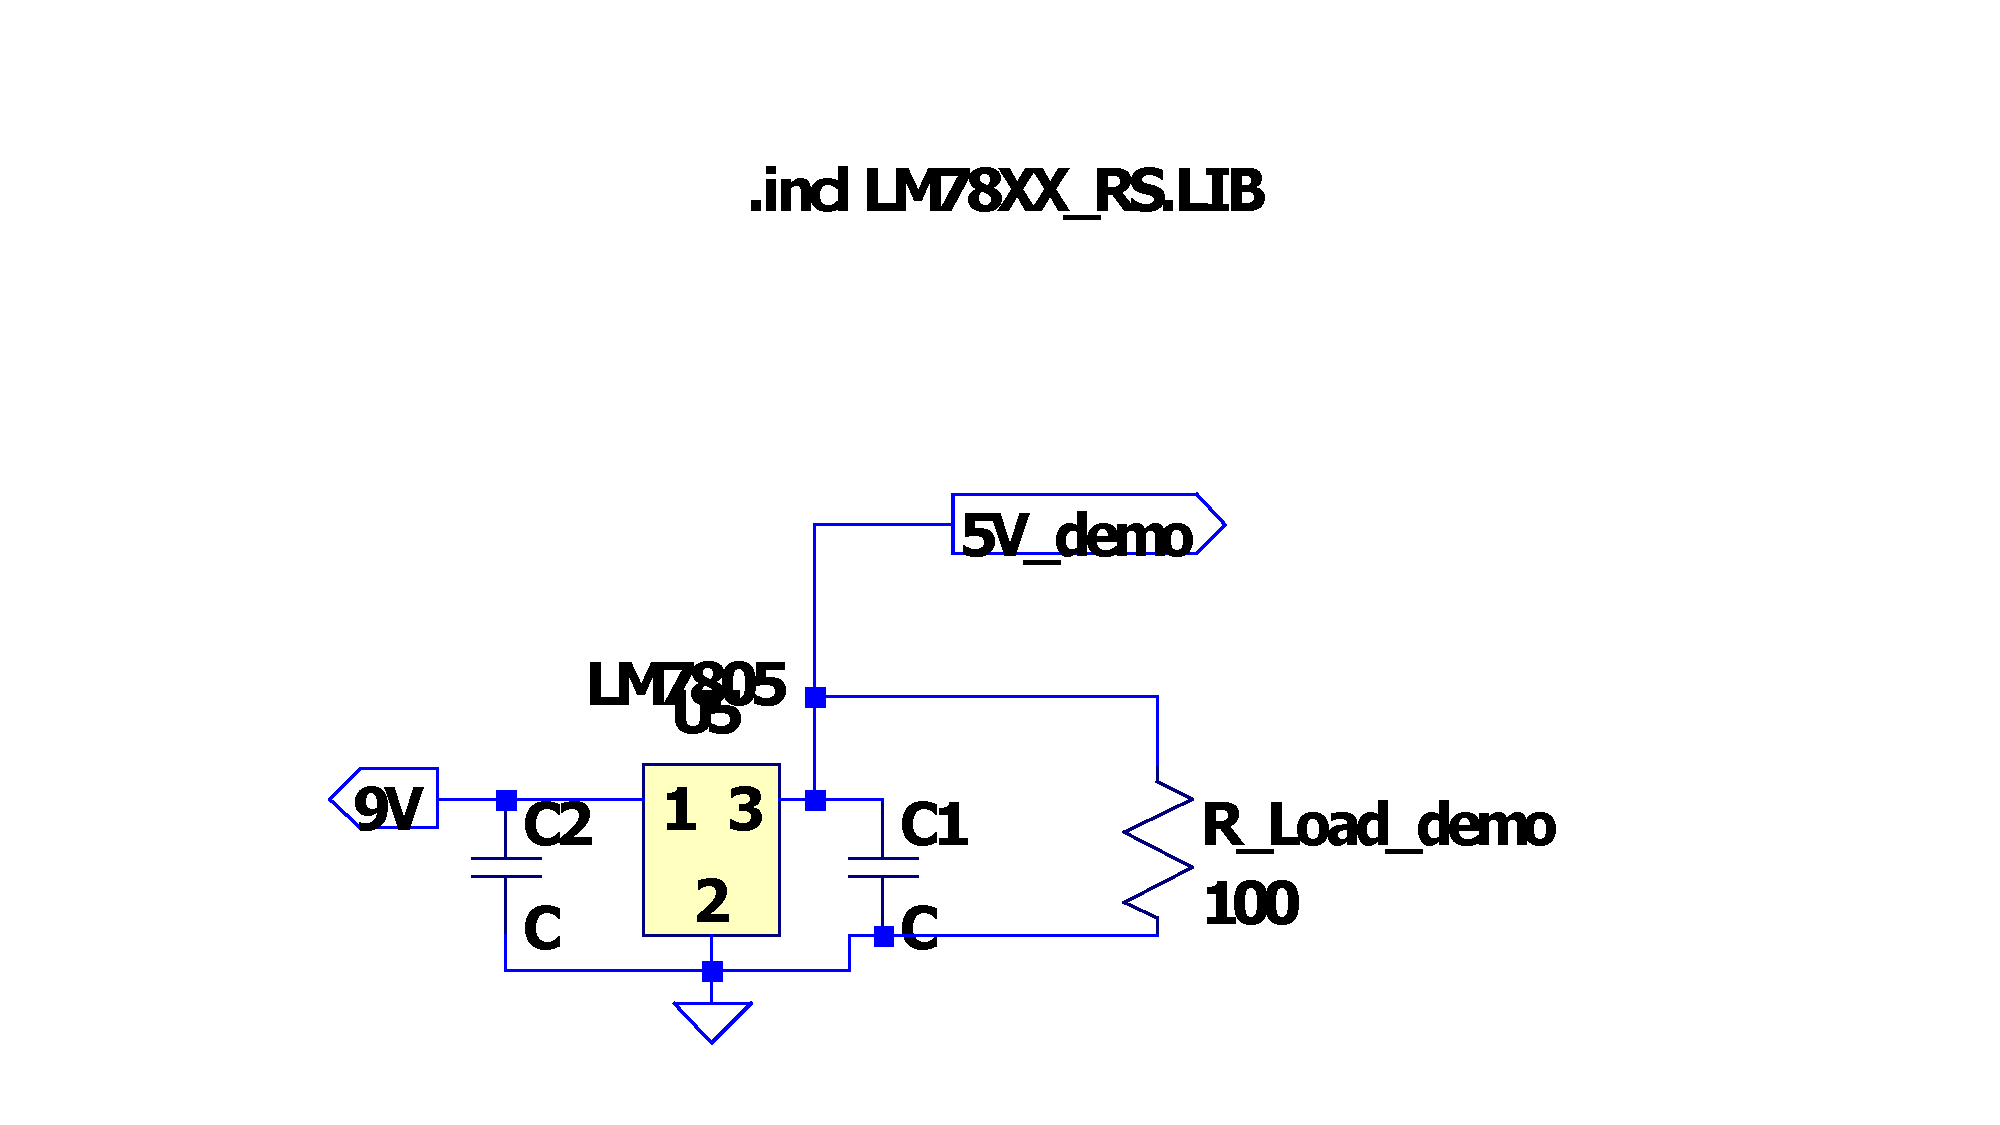
\includegraphics[width=\linewidth]{./Figures/E344_Ass1VoltRegulator_cct}
	  \caption{Linear voltage regulator.} \label{subfig:linear_circuit_diagram}	
   \end{subfigure}
   \begin{subfigure}[]{0.45\textwidth}
  	 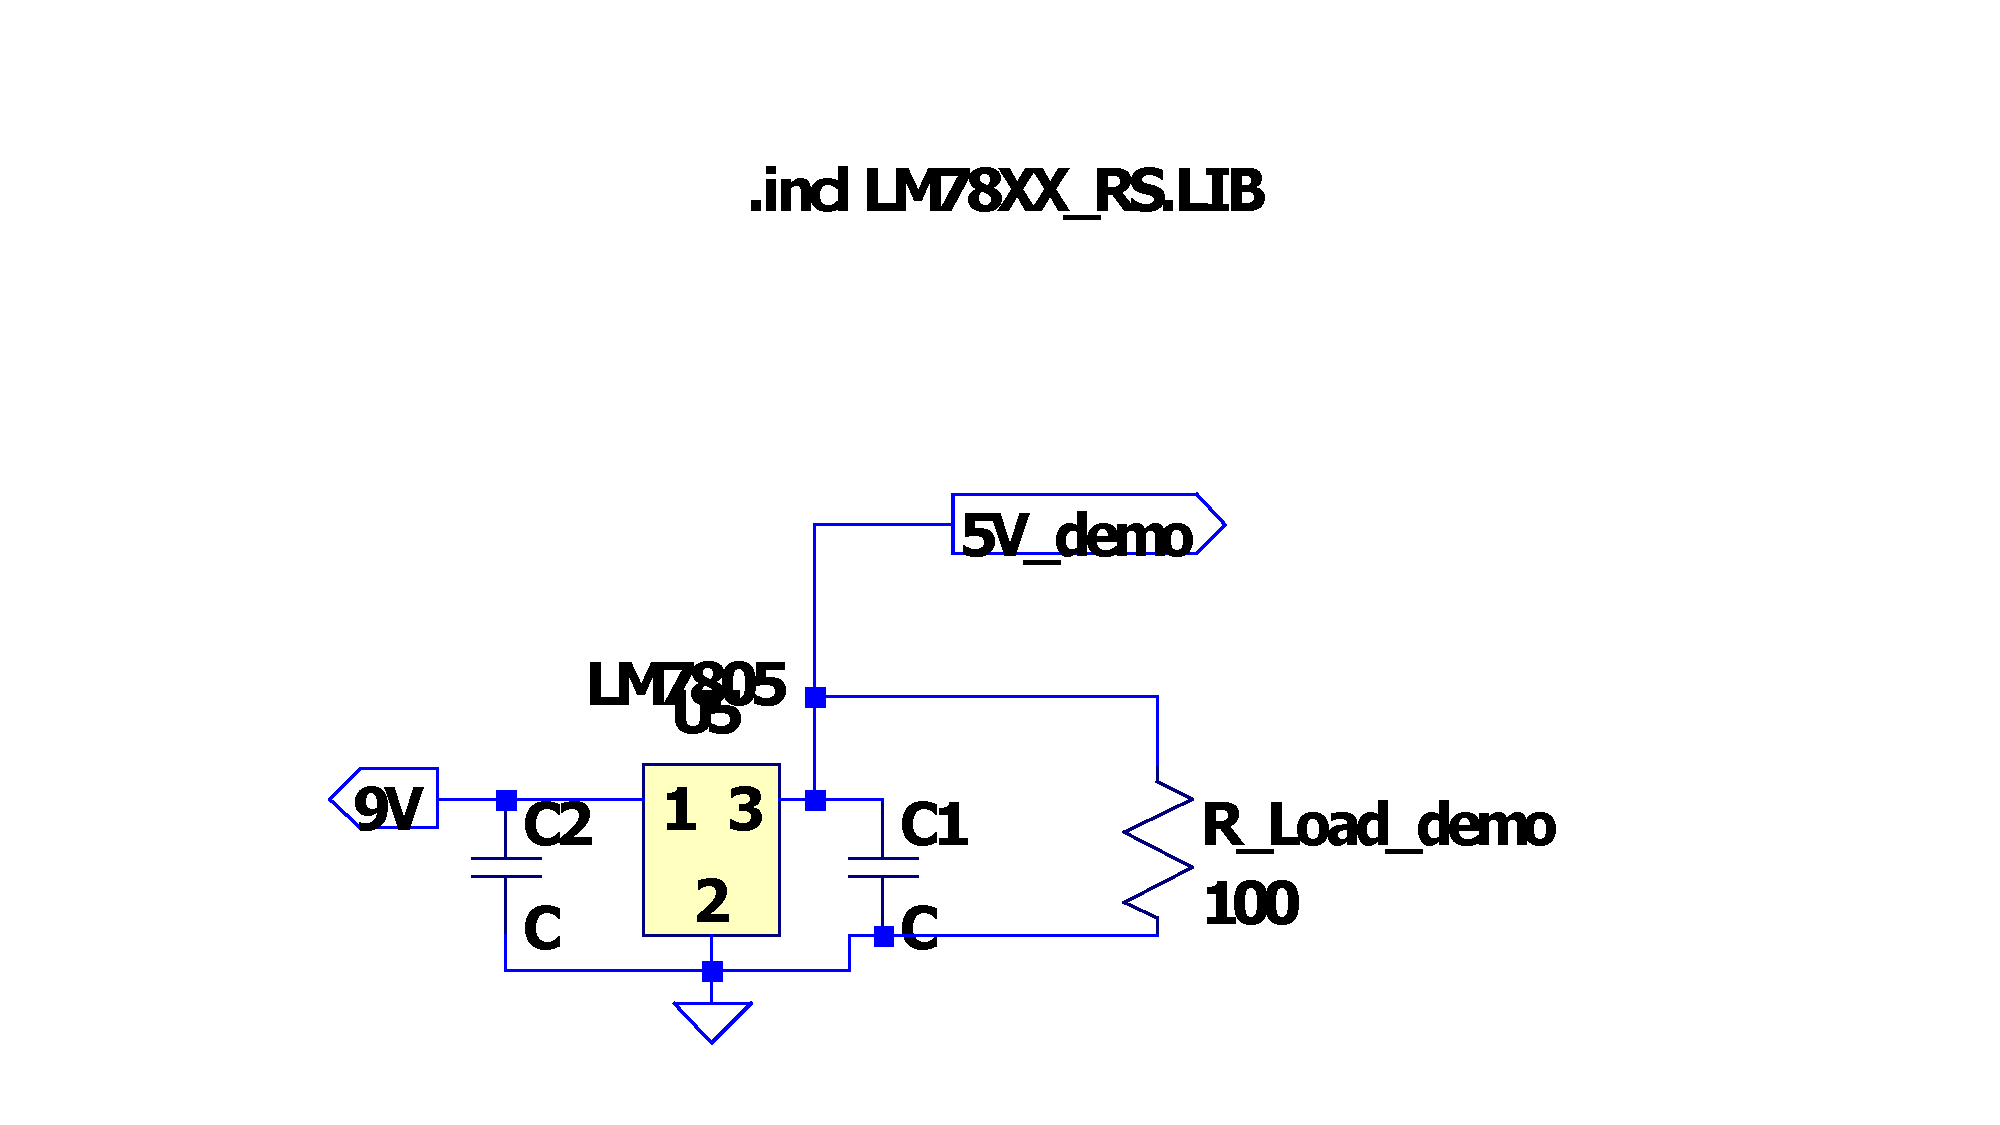
\includegraphics[width=\linewidth]{./Figures/E344_Ass1VoltRegulator_cct}
	  \caption{Switchmode voltage regulator.} \label{subfig:switchmode_circuit_diagram}	
   \end{subfigure}
   \begin{subfigure}[]{0.95\textwidth}
  	 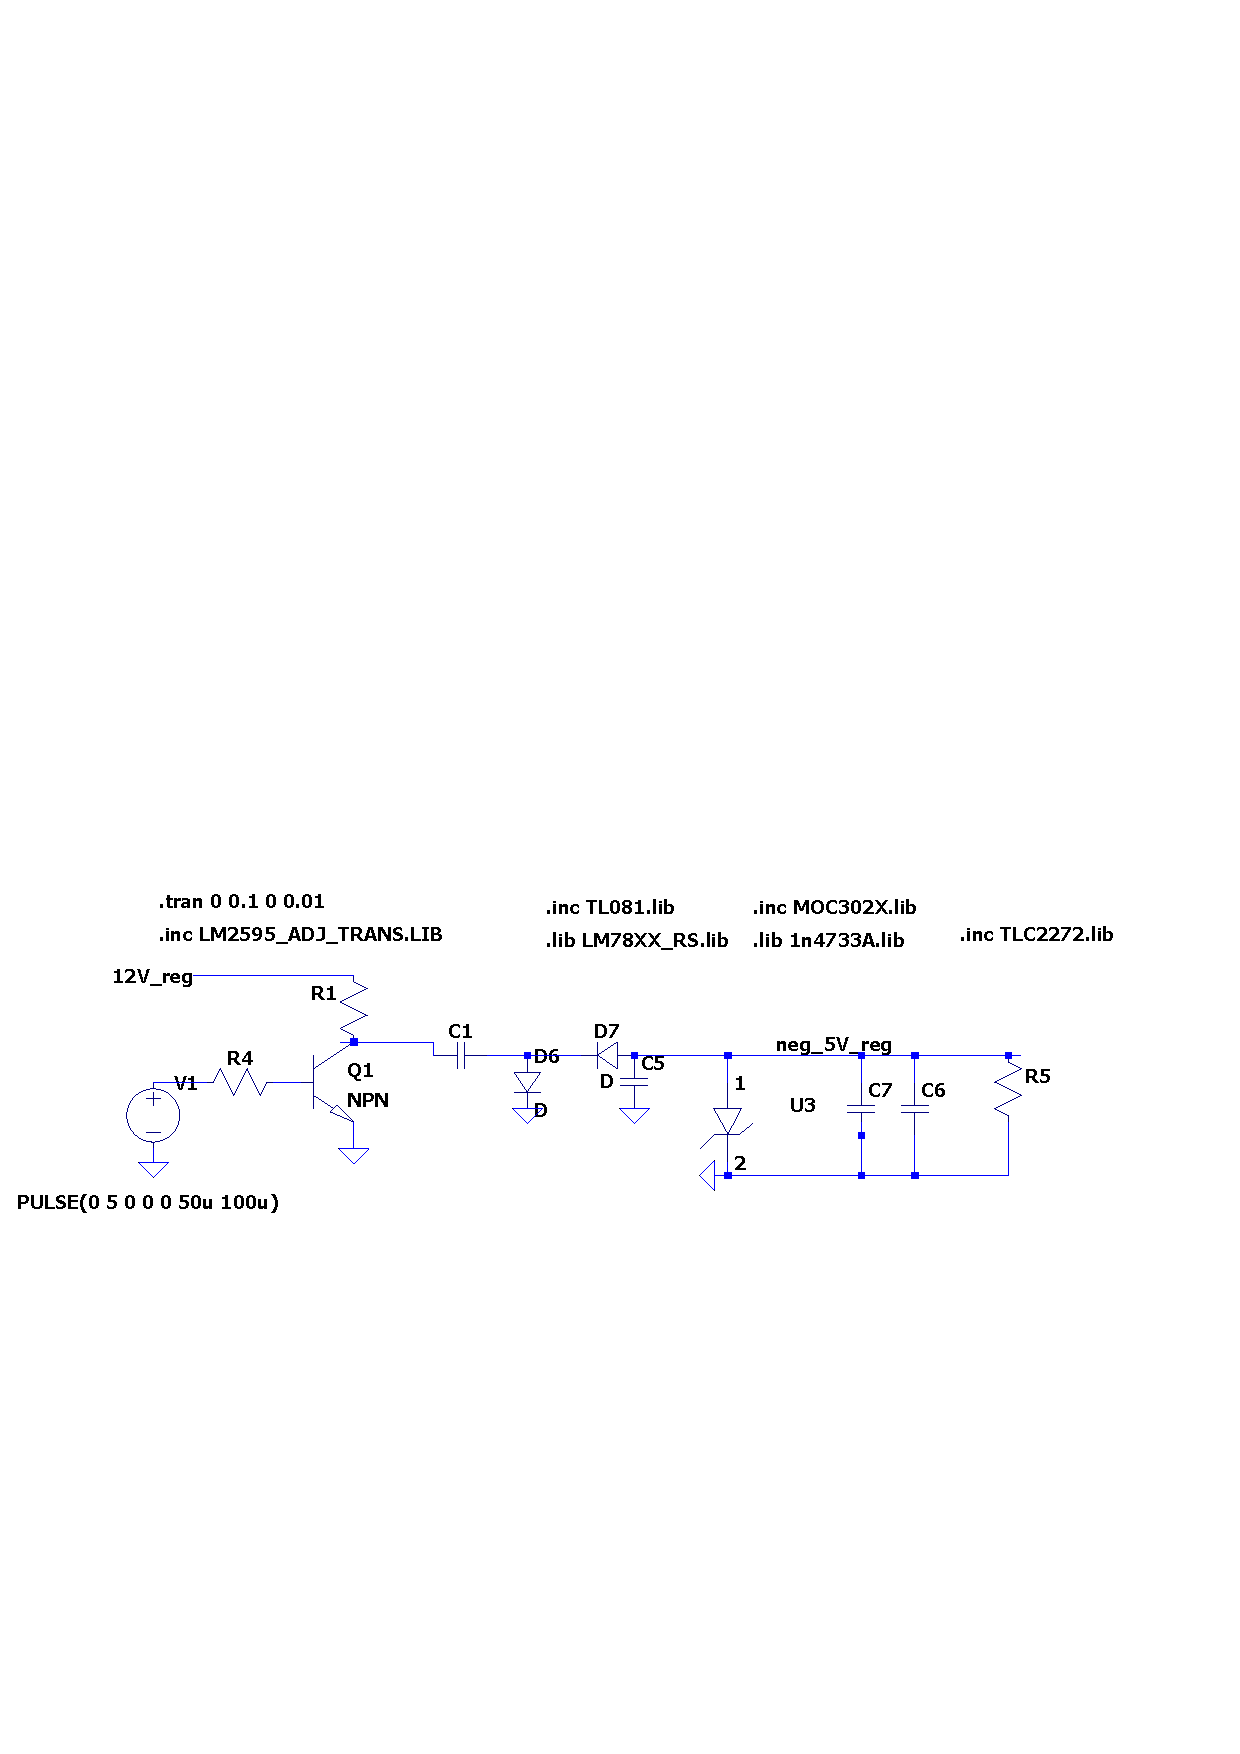
\includegraphics[width=\linewidth]{./Figures/CctDia}
	  \caption{Chargepump voltage regulator.} \label{subfig:chargepump_circuit_diagram}	
   \end{subfigure}
   
   \caption {Circuit diagrams of the two voltage regulators, and another irrelevant one}.

      \label{fig:circuit_diagram}
 \end{figure}
%**********************************************
\section{Results} \label{sec:heartResults}
%**********************************************


\begin{figure}
 \footnotesize
 \centering
    \begin{subfigure}[]{0.55\textwidth}
              \centering
  		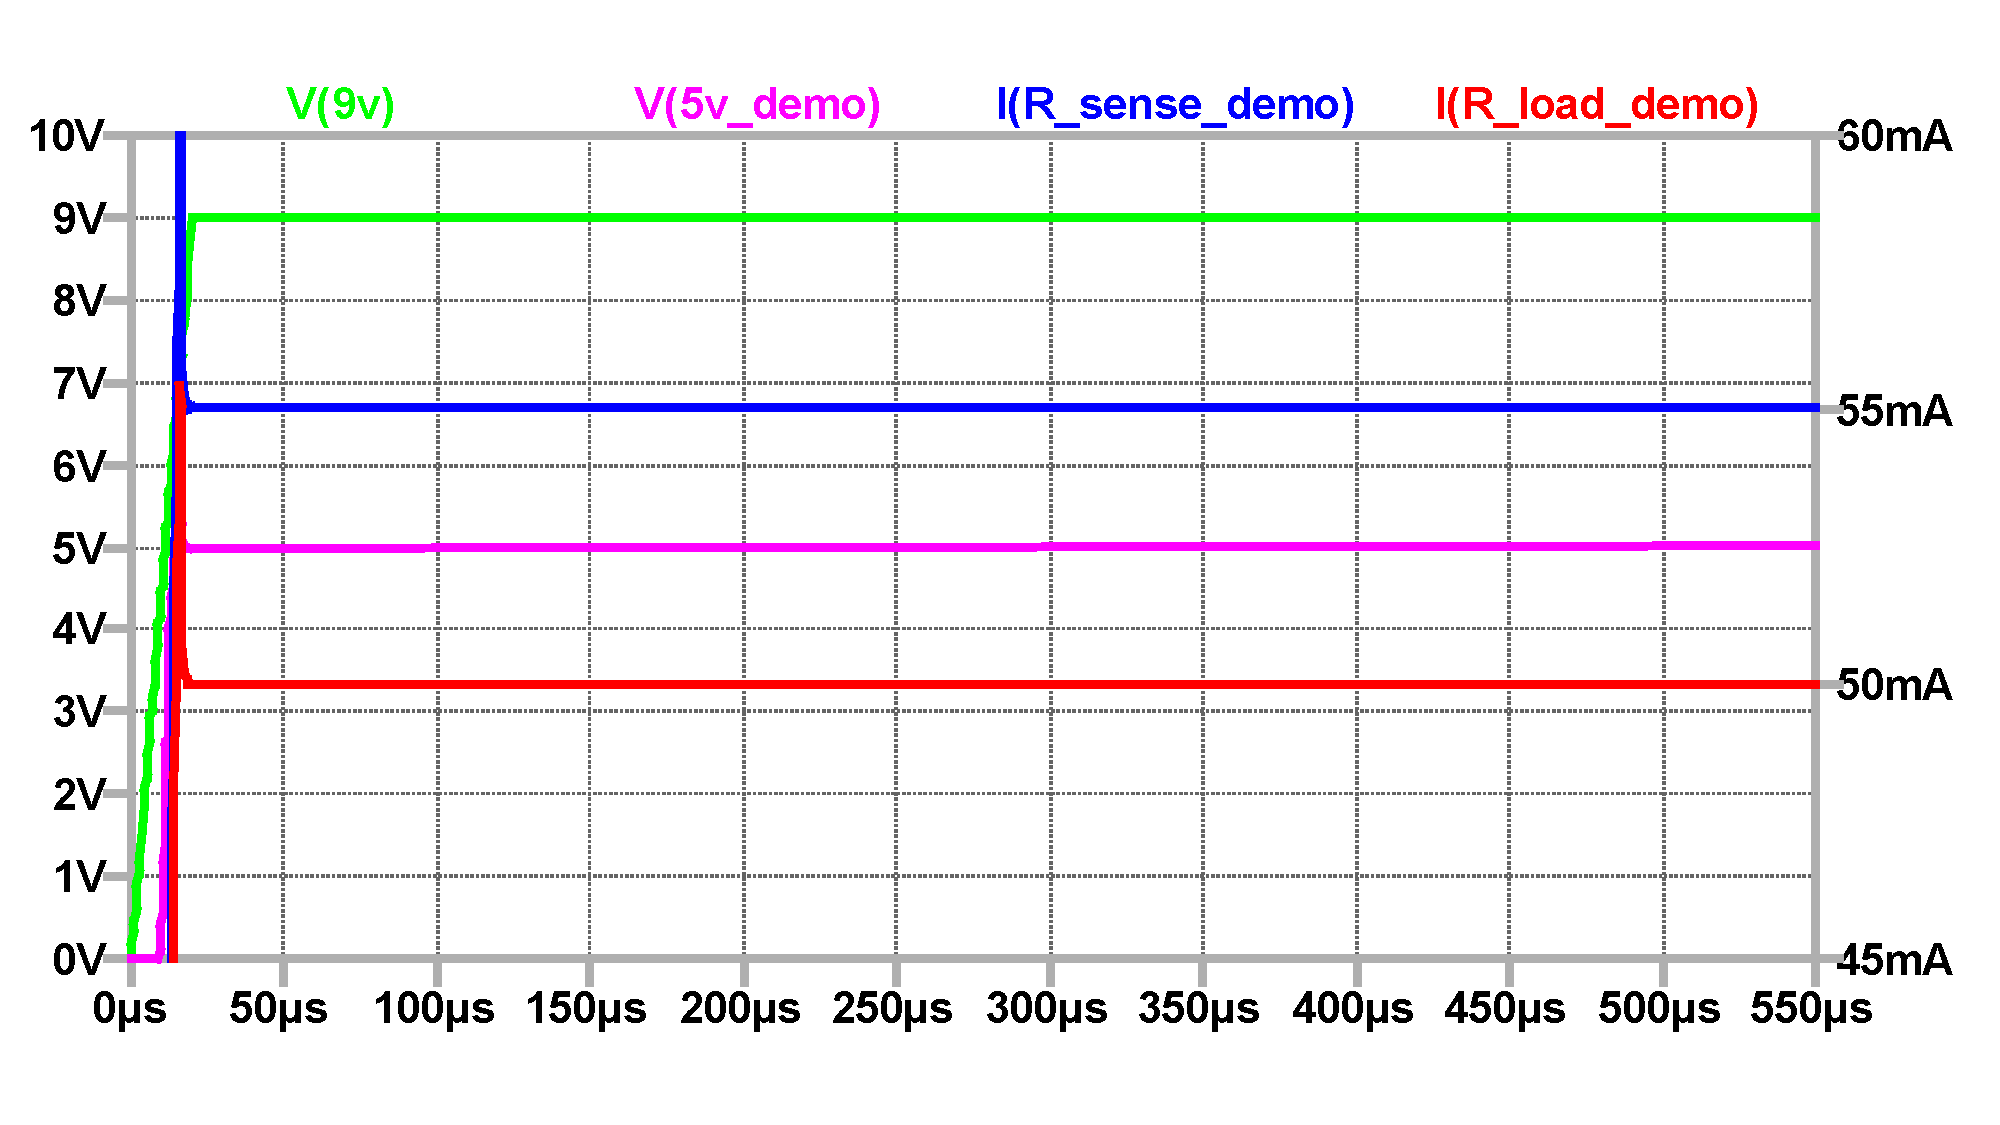
\includegraphics[width=1\linewidth]{./Figures/E344_VoltRegulator.pdf}
		    \caption{} \label{subfig:pwr_simu_rect}
     \end{subfigure}
     \begin{subfigure}[]{0.4\textwidth}
             \centering
  		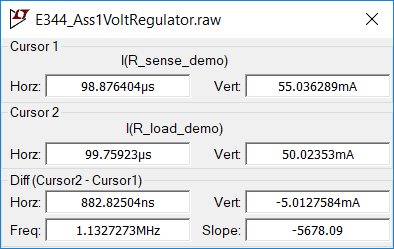
\includegraphics[width=1.0\linewidth]{./Figures/Screengrab2}
		   \caption{ } \label{subfig:pwr_meas_rect}
     \end{subfigure}
    \begin{subfigure}[]{0.55\textwidth}
              \centering
  		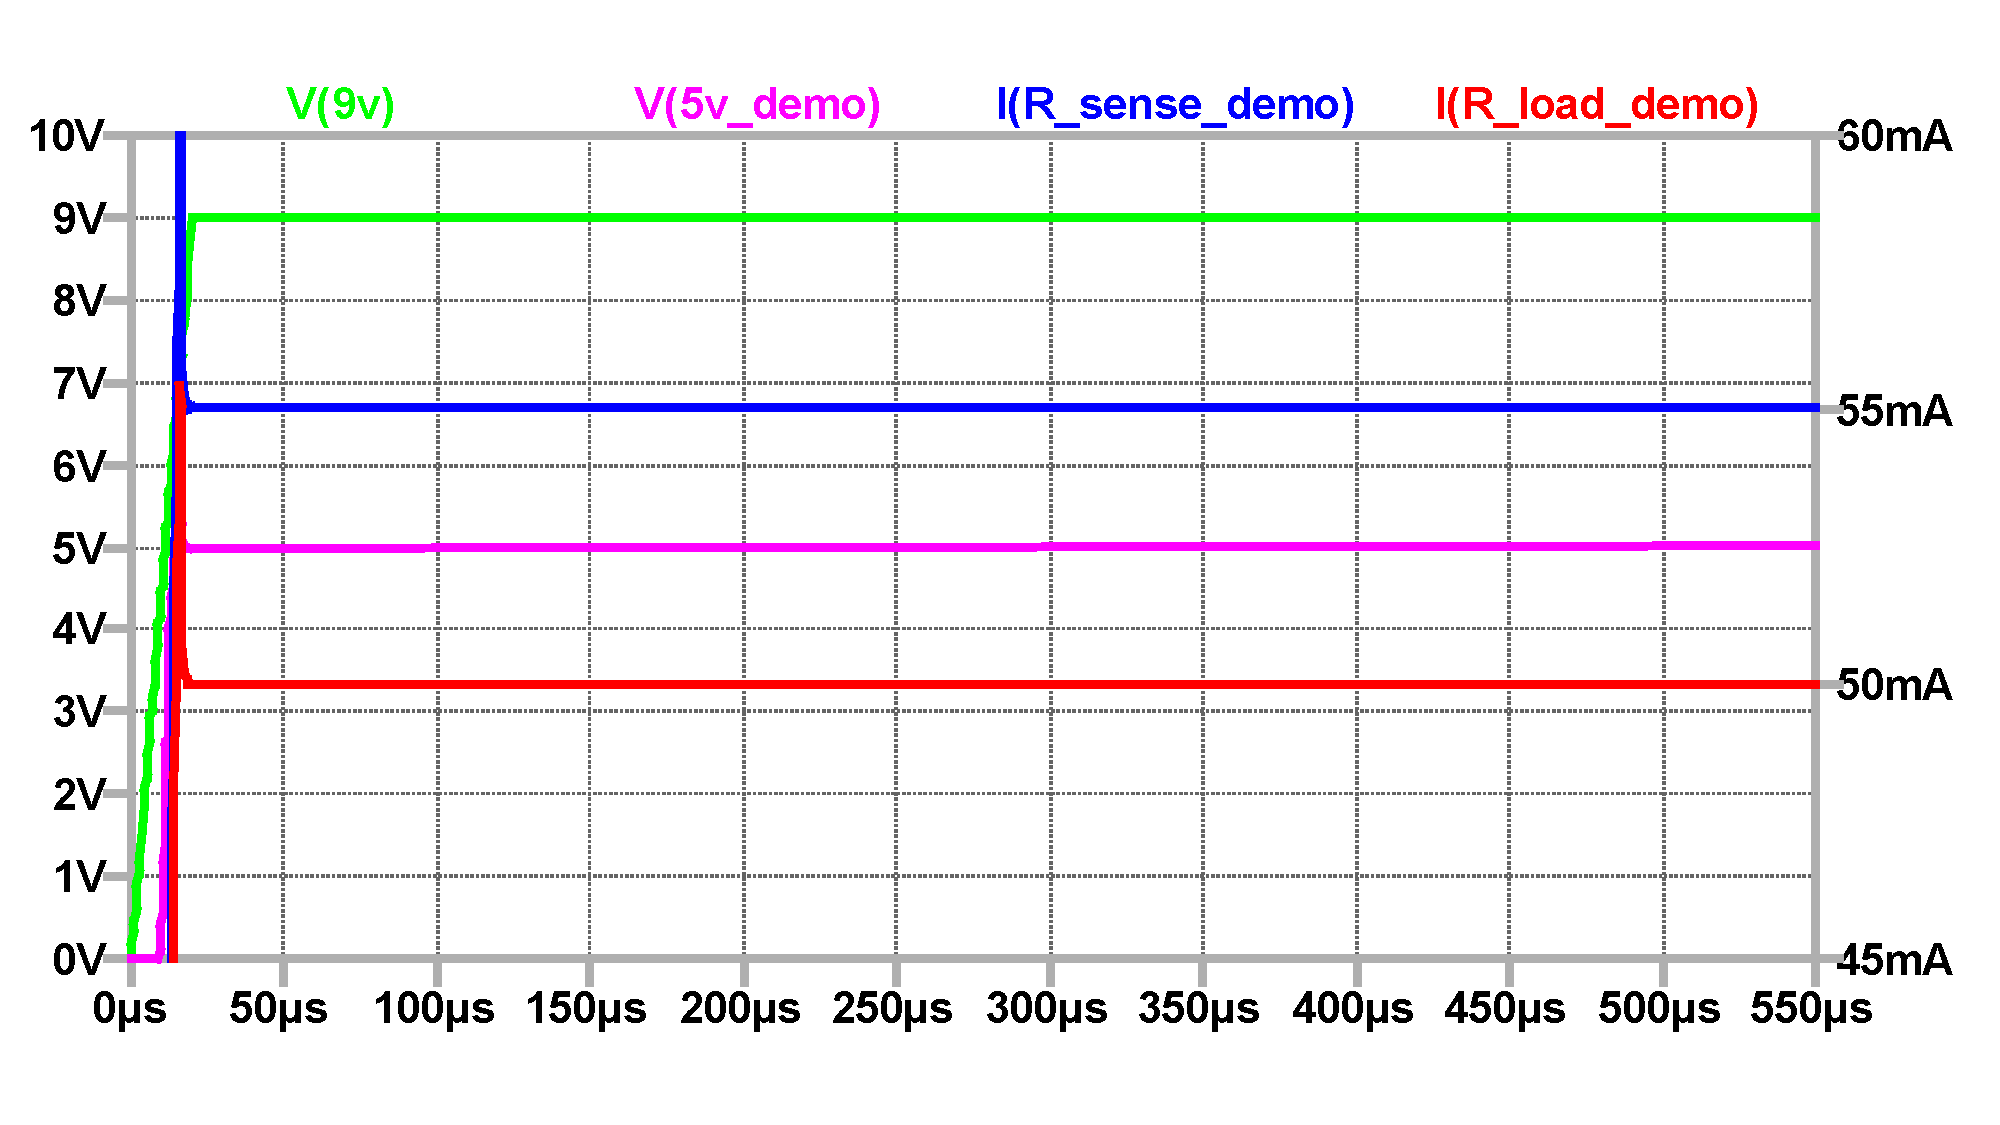
\includegraphics[width=1\linewidth]{./Figures/E344_VoltRegulator.pdf}
		    \caption{} \label{subfig:pwr_simu_rect}
     \end{subfigure}
    \begin{subfigure}[]{0.4\textwidth}
              \centering
  		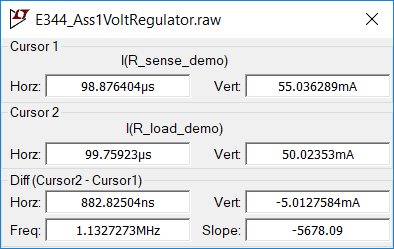
\includegraphics[width=1\linewidth]{./Figures/Screengrab2}
		    \caption{} \label{subfig:pwr_simu_rect}
     \end{subfigure}
   \caption[\textcolor{red}{I am the short caption that appears in the List of Figures list}]{Voltage regulation, comparing the linear and switchmode regulators... (a)  Blah blah. (b)  Blah blah.  (c)  Blah blah. (d) Blah blah.   As far as possible, please put input(s) and output(s) on the same plot rather than on separate plots. Based on the datasheet of XXXX in \cite{WebsiteOpAmp}}
    \label{fig:simulation_results_box}
 \end{figure}

In this section, you want to demonstrate, by means of referring to simulation results, using the designed circuit, how your circuit behaves as you designed it in Section \ref{sec:heartDesign}. Present and report on your simulated results in Figure \ref{fig:simulation_results_box}. Be absolutely sure that the text and information in your report are readable. 

You can use screengrabs or photos of the oscilloscope, or download the CSVs and plot them as PDFs using Matlab, Excel or similar. 
You can also use tables, example of which are presented in Tables \ref{tab:table1} and \ref{tab:table2}.


\begin{table}
        \centering
        \footnotesize
        \caption{Example of a simple table.}
         \begin{tabular}{c@{\qquad}rrrr}
          \toprule
             & 2017 & 2018 & $\Delta_{Abs}$ & $\Delta_{DiD}$\\
          \midrule
          A & 9,868      & 10,399 & +5 & -11\\
          B & 10,191     & 10,590 & +4 & -12\\
          \bottomrule
        \end{tabular}
     \label{tab:table1}
\end{table}


\begin{table}
         \centering
        \footnotesize
        \caption{Example of another table.}

         \begin{tabular}{c@{\qquad}rrrr}
          \toprule
          \multirow{2}{*}{\raisebox{-\heavyrulewidth}{Schools }} & \multicolumn{2}{c}{Total energy used}& \multicolumn{2}{c}{Change}\\
          \cmidrule{2-5}
            & 2017 & 2018 & $\Delta_{Abs}$ & $\Delta_{DiD}$\\
            & [kWh] & [kWh] & [\%] & [\%] \\
          \midrule
          A & 9,868      & 10,399 & +5 & -11\\
          B & 10,191     & 10,590 & +4 & -12\\
          \bottomrule
        \end{tabular}
     \label{tab:table2}
\end{table}


%**********************************************
\section{Summary}\label{sec:temp_summary}
%**********************************************
State whether your design performs as expected and what the limitations are or things to keep in mind are. 


